\documentclass[12pt]{article}

\usepackage[utf8]{inputenc}
\usepackage[english, russian]{babel}

\usepackage{slides}
\usepackage{tikz}
\usepackage{pgfplots}

\IfFileExists{cyrtimes.sty}
    {
        \usepackage{cyrtimespatched}
    }
    {
    }

\usepackage{graphicx}
\def\Student{Романов Алексей Сергеевич}
\def\Advisor{Рудаков Игорь Владимирович}
\def\Title{Анализ UML диаграмм деятельности с помощью раскрашенных сетей Петри}
% Титул для нижнего колонтитула. Может быть сокращённым
\def\FooterTitle{\Title}
\def\SubTitle{Дипломная работа}
\newcommand{\TitleSlide}{
    \addcontentsline{toc}{section}{\Title}%
    ~\vspace{1cm}

    \begin{center}
    {\huge \begin{spacing}{1}\Title\end{spacing}}

    {\SubTitle}
    \vspace{2cm}

    \ifthenelse{\isundefined{\Student}}{}
        {\small Студент: \Student\\}
    \ifthenelse{\isundefined{\Advisor}}{}
        {\small Руководитель: \Advisor\\}
    \ifthenelse{\isundefined{\Person}}{}
        {\Person\\}
    \ifthenelse{\isundefined{\Affilation}}{}
        {\Affilation\\}
    \end{center}
    \thispagestyle{empty}
}


%% Переносы в презентации смотряся не очень.
\hyphenpenalty 10000
\sloppy


\begin{document}

\TitleSlide

\section{Цели и решаемые задачи}

\emph{Целью работы} является разработка метода представления диаграммы деятельности раскрашенной сетью Петри, позволяющего выявить блокировки и недостижимые состояния.

\emph{Решаемые задачи}
\begin{small}
	\begin{enumerate}
	\item[1.] Классифицировать существующие методы анализа диаграмм деятельности.
	\item[2.] Разработать метод представления диаграммы деятельности в виде раскрашенной сети Петри.
	\item[3.] Программно реализовать метод представления диаграммы деятельности в виде раскрашенной сети Петри.
	\item[4.] Исследовать факторы, влияющие на появление блокировок.
	\item[5.] Исследовать корректность построения раскраски сети.
	\end{enumerate}
\end{small}

\section{Классификация методов анализа диаграмм деятельности}

\begin{center}
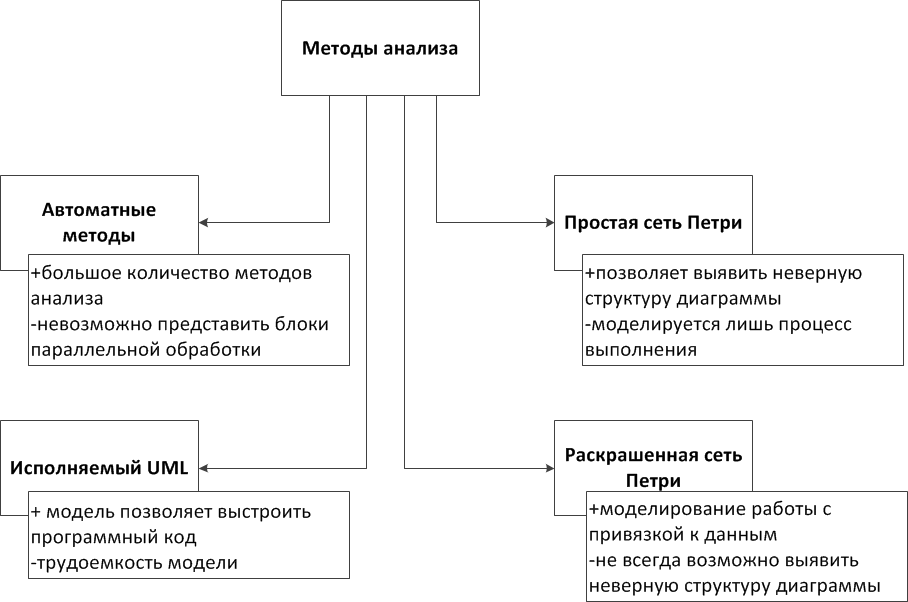
\includegraphics[scale=0.85]{../tex/include/MethodClassification.png}
\end{center}

\section{Функциональная модель метода}

\begin{center}
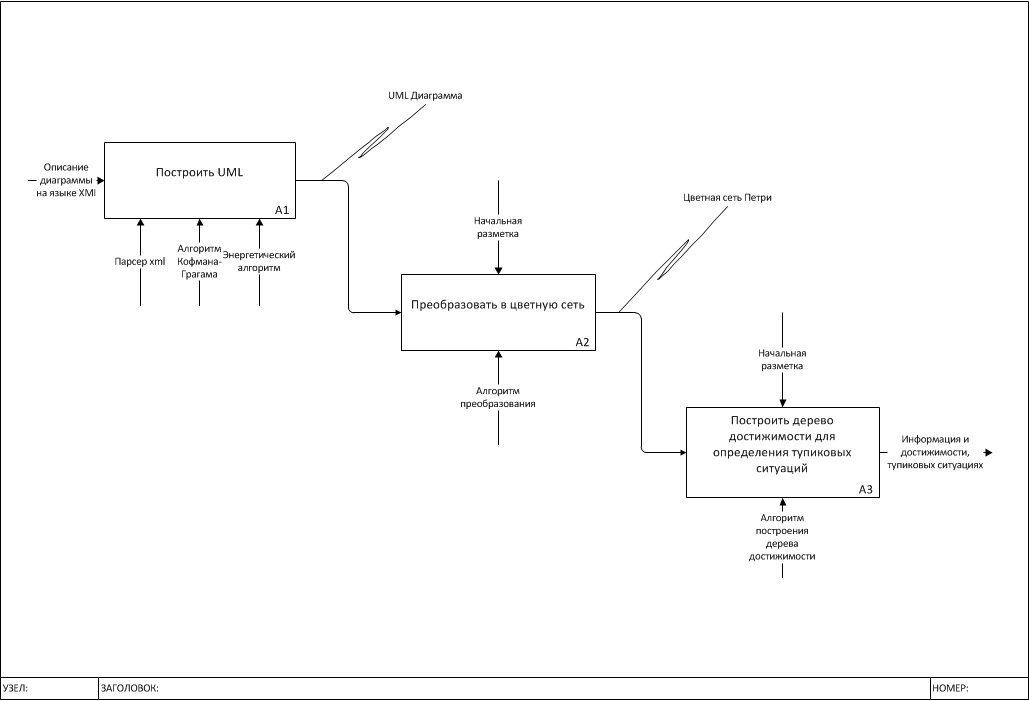
\includegraphics[width=\textwidth]{../tex/include/IDEF0.png}
\end{center}

\section{Представление UML диаграмм}

\begin{minipage}[H]{0.48\linewidth}
UML := (XMI (XML) | OMG), где \\
XMI ~--- XML Mmetadata Interchange \\
XML ~--- eXtensible Markup Language \\
OMG ~--- Object Management Group

\end{minipage}
\hfill
\begin{minipage}[H]{0.55\linewidth}
	\begin{small}
		\begin{verbatim}
<activity_diagram>
    <states>
        <state id, name, type>
            <incoming transitions>
            <outgoing transition>
            <action>
        </state>
    </states>
    <transitions>
        <transition id>
            <source state>
            <target state>
            <guard>
        </transition>
    </transitions>
<activity_diagram>
		\end{verbatim}
	\end{small}
\end{minipage}

\section{Отображение диаграммы деятельности}

Представим диаграмму деятельности в виде ориентированого графа $ G = (V, E) $, где \\
$ V = (v_{1} ... v_{k}), v_{i} $ ~--- вершина графа; \\
$ E = (e_{1} ... e_{n}), e_{i} $ ~--- переход между вершинами.

Алгоритм отображения состоит из трех этапов.
\begin{enumerate}
\item[1.] Построение ассоциированного орграфа.
\item[2.] Топологическая сортировка вершин исходного и ассоциированного графа.
\item[3.] Мозаичное и полилинейное представление.
\end{enumerate}

\section{Построение ассоциированного орграфа}

Ассоциированный с графом G граф $ G^{*} = (V^{*}, E^{*}) $, где \\
$ V^{*} : v \epsilon F $ \\
$ E^{*} : \forall e \epsilon E : e^{*} = (f, g), f = left(e), g = right(e) $

\begin{figure}[h!]
	\begin{minipage}[H]{0.32\linewidth}
		\center{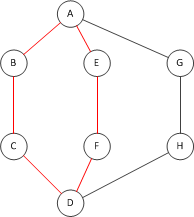
\includegraphics[scale=1]{../tex/include/RemoveCycles1.png} \\ \tiny Цикл (A,B) \rightarrow (B,C) \rightarrow (C,D) \rightarrow (D,F) \rightarrow (F,E) \rightarrow (E,A)}
	\end{minipage}
	\hfill
	\begin{minipage}[H]{0.32\linewidth}
		\center{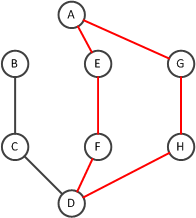
\includegraphics[scale=1]{../tex/include/RemoveCycles2.png} \\ \tiny Цикл (A,E) \rightarrow (E,F) \rightarrow (F,D) \rightarrow (D,H) \rightarrow (H,G) \rightarrow (G,A)}
	\end{minipage}
	\hfill
	\begin{minipage}[H]{0.32\linewidth}
		\center{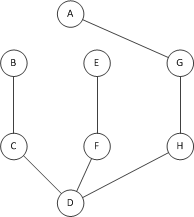
\includegraphics[scale=1]{../tex/include/RemoveCycles3.png} \\ \tiny  Циклов нет }
	\end{minipage}
\end{figure}

\section{Мозаичное представление графа}

\begin{minipage}[H]{0.49\linewidth}
	\center{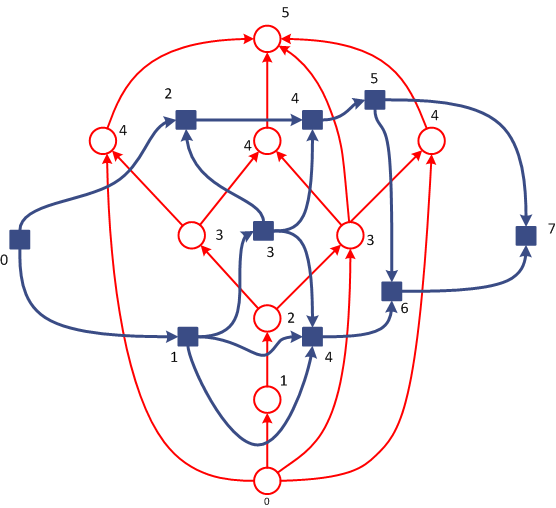
\includegraphics[scale=0.9]{../tex/include/Graph.png}}
	\caption{\begin{small}Граф G (красный) и ассоциированный орграф G* (синий).\end{small}}
\end{minipage}
\hfill
\begin{minipage}[H]{0.49\linewidth}
	\center{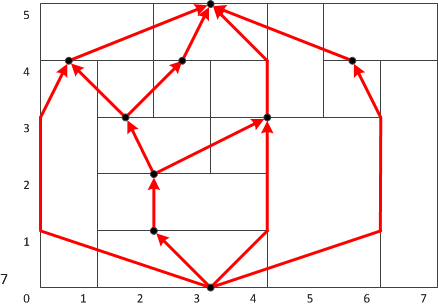
\includegraphics[scale=0.9]{../tex/include/PolylineView.png}}
	\caption{\begin{small}Полилинейное представление графа G.\end{small}}
\end{minipage}

\section{Раскрашенные сети Петри}

Раскрашенная сеть Петри $ CPN = (\Sigma, P, T, A, N, C, G, E, I) $, где \\
$ \Sigma $ ~--- конечное непустое множество цветов; \\
P ~--- конечное множество позиций; \\
T ~--- конечное множество состояний; \\
A ~--- конечное множество дуг, таких что $ P \cap T = P \cap A = T \cap A = 0 $; \\
N ~--- позиционная функция, отображающая A в  $ P \times T \cup T \times P $; \\
C ~---функция раскраски, отображающая P в $ \sigma $; \\
G ~---защита переходов, отображающая T в выражение вида $ \forall t \epsilon T : [Type(G(t)) = bool & Type(Var(G(t))) \subseteq \Sigma] $; \\
E ~--- выражения на дугах, отображающая A в выражение вида $ \forall a \epsilon A : [Type(E(a)) = C(p(a))_{ms} & Type(Var(E(a))) \subseteq \Sigma] $, где p(a) ~--- позиция N(a); \\
I ~--- функция инициализации, отображающая P в выражение вида $ \forall p \epsilon P : [Type(I(p)) = C(p)_{ms}] $.

\section{Этапы построения раскрашенной сети Петри}

\begin{center}
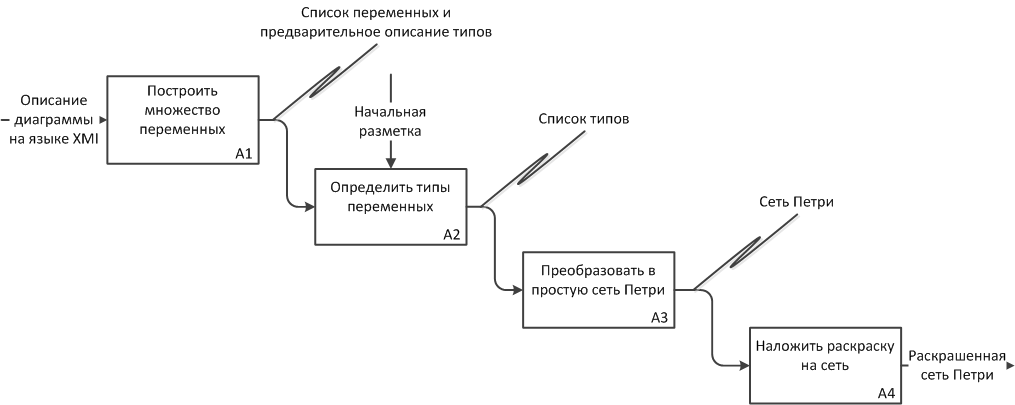
\includegraphics[width=\textwidth]{../tex/include/IDEF0ColoredPetri.png}
\end{center}

\section{Преобразование диаграммы деятельности в раскрашенную сеть Петри (1)}

\begin{minipage}[H]{0.55\linewidth}
	\center{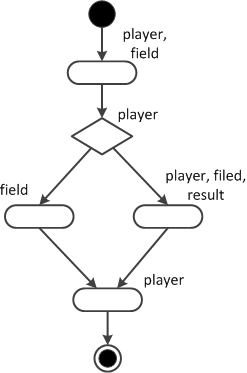
\includegraphics[scale=1.3]{../tex/include/ConvertVariables.png}}
\end{minipage}
\hfill
\begin{minipage}[H]{0.44\linewidth}
	\begin{enumerate}
	\item[1.] Разбор выражений.
	\item[2.] Выделение списка переменных для каждой вершины.
	\end{enumerate}
\end{minipage}

\section{Преобразование диаграммы деятельности в раскрашенную сеть Петри (2)}

\begin{minipage}[H]{0.55\linewidth}
	\center{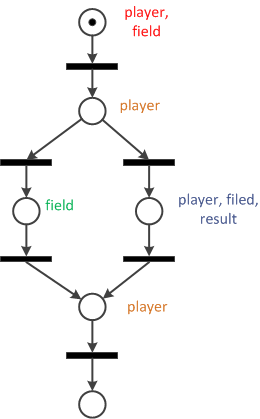
\includegraphics[scale=1.2]{../tex/include/ConvertDiagram.png}}
\end{minipage}
\hfill
\begin{minipage}[H]{0.44\linewidth}
	\begin{enumerate}
	\item[1.] Преобразование диаграммы деятельности в простую сеть Петри.
	\item[2.] Формирование множества типов переменных.
	\item[3.] Предварительное определение множества раскрасок.
	\end{enumerate}
\end{minipage}

\section{Преобразование диаграммы деятельности в раскрашенную сеть Петри (3)}

\begin{minipage}[H]{0.55\linewidth}
	\center{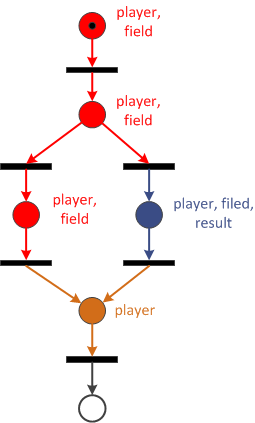
\includegraphics[scale=1.2]{../tex/include/ConvertColoring.png}}
\end{minipage}
\hfill
\begin{minipage}[H]{0.44\linewidth}
	\begin{enumerate}
	\item[1.] Определение максимальной области видимости переменных.
	\item[2.] Формирование результирующей раскраски.
	\end{enumerate}
\end{minipage}

\section{Исследование причин возникновения блокировок}

Причины возникновения блокировок:

\begin{itemize}
\item неверная структура диаграммы;
\item невозможность перехода из-за невыполнения логичского условия спусковой функции.
\end{itemize}

\begin{minipage}[H]{0.22\linewidth}
	\center{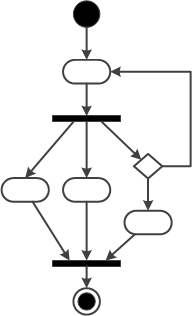
\includegraphics[scale=1]{../tex/include/BlockedDiagram1.png}}
\end{minipage}
\hfill
\begin{minipage}[H]{0.22\linewidth}
	\center{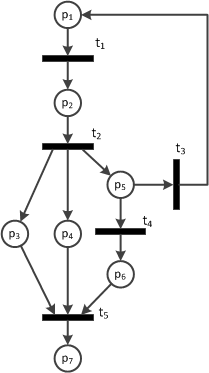
\includegraphics[scale=1]{../tex/include/BlockedNet1.png}}
\end{minipage}
\hfill
\begin{minipage}[H]{0.01\linewidth}
\begin{tikzpicture}
	\draw (0, - 4.5) -- (0, 4.5);
\end{tikzpicture}
\end{minipage}
\hfill
\begin{minipage}[H]{0.22\linewidth}
	\center{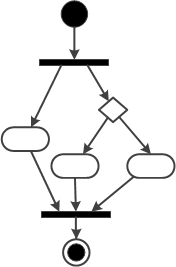
\includegraphics[scale=1]{../tex/include/BlockedDiagram2.png}}
\end{minipage}
\hfill
\begin{minipage}[H]{0.22\linewidth}
	\center{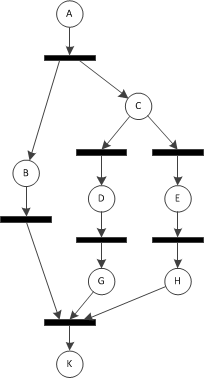
\includegraphics[scale=1]{../tex/include/BlockedNet2.png}}
\end{minipage}

\section{Исследование корректности построения раскраски сети}

\begin{minipage}[H]{0.45\linewidth}
Два подхода к построению раскраски:
\begin{itemize}
\item[1.] определять раскраску всех элементов цикла как кортеж переменных наибольшей мощности;
\item[2.] определять раскраску не учитывая обратную дугу цикла.
\end{itemize}
\end{minipage}
\hfill
\begin{minipage}[H]{0.26\linewidth}
	\center{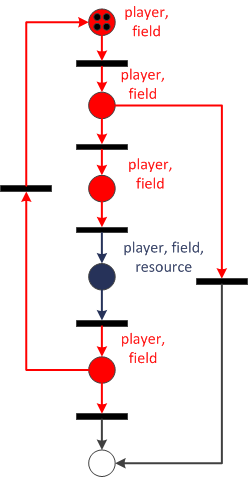
\includegraphics[scale=0.9]{../tex/include/ResearchWithCycle.png}}
\end{minipage}
\hfill
\begin{minipage}[H]{0.26\linewidth}
	\center{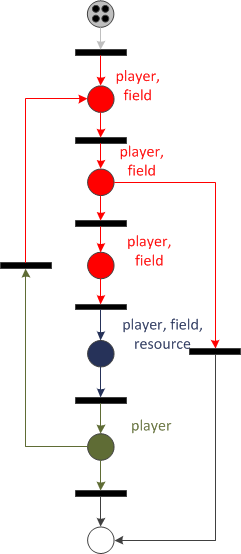
\includegraphics[scale=0.9]{../tex/include/ResearchWithoutCycle.png}}
\end{minipage}

\section{Сравнение скорости работы простой и раскрашенной сети Петри}

\begin{center}
	\begin{tikzpicture}
		\begin{axis}[width=22cm, compat=newest, xtick={8,10,...,28}, height=12cm, grid=major, xmin=8, xmax=28, ymin=0,  xlabel=Количество состояний, ylabel=Время моедлирования (мс), no markers]
		\addplot+[smooth] coordinates
		{ (8, 12) (12, 14) (15, 15) (20, 18) (25, 20) (28, 23) };
		\addlegendentry{Простая сеть}
		\addplot+[smooth] coordinates
		{ (8, 45) (12, 56) (15, 67) (20, 89) (25, 113) (28, 143) };
		\addlegendentry{Раскрашенная сеть}
		\end{axis}
	\end{tikzpicture}
\end{center}

\section{Сравнение количества затраченных ресурсов для простой и раскрашенной сети Петри}

\begin{center}
	\centering
	\begin{tikzpicture}
		\begin{axis}[width=22cm, compat=newest, xtick={8,10,...,28}, height=12cm, grid=major, xmin=8, xmax=28, ymin=0, xlabel=Количество состояний, ylabel=Количество ресурсов, no markers]
		\addplot+[smooth] coordinates
		{ (8, 250) (12, 310) (15, 340) (20, 475) (25, 585) (28, 612) };
		\addlegendentry{Простая сеть}
		\addplot+[smooth] coordinates
		{ (8, 345) (12, 390) (15, 420) (20, 655) (25, 730) (28, 795) };
		\addlegendentry{Раскрашенная сеть}
		\end{axis}
	\end{tikzpicture}
\end{center}

\section{Выводы}

\begin{enumerate}
\item[1.] Проведена классифицкация существующих методов анализа диаграмм деятельности.
\item[2.] Разработан метод представления диаграммы деятельности в виде раскрашенной сети Петри.
\item[3.] Разработано программное обеспечение, реализующее предложенный метод.
\item[4.] Исследованы факторы, влияющие на появление блокировок.
\item[5.] Исследована корректность построения раскраски сети.
\end{enumerate}

\end{document}

